\documentclass[10pt, conference]{IEEEtran}

\usepackage{mdframed,graphicx,booktabs,textcomp,multirow,pgfplots,cite}
\usepackage{graphicx}

\pgfplotsset{
    integral segments/.code={\pgfmathsetmacro\integralsegments{#1}},
    integral segments=3,
    integral/.style args={#1:#2}{
        ybar interval,
        domain=#1+((#2-#1)/\integralsegments)/2:#2+((#2-#1)/\integralsegments)/2,
        samples=\integralsegments+1,
        x filter/.code=\pgfmathparse{\pgfmathresult-((#2-#1)/\integralsegments)/2}
    }
}


\ifCLASSINFOpdf
 
\else
\fi

\hyphenation{Bug Fix Verification An Analysis of Pull Request Acceptance on the Tree-Structured Level}

\begin{document}
%
% paper title
% can use linebreaks \\ within to get better formatting as desired
\title{Bug Fix Verification: An Analysis of Pull Request Acceptance on the Tree-Structured Level}


% author names and affiliations
% use a multiple column layout for up to two different
% affiliations

\author{\IEEEauthorblockN{Yu-Ann Chen}
\IEEEauthorblockA{Institute of Software Research\\Carnegie Mellon University\\yuannc@andrew.cmu.edu}
}
\maketitle


\begin{abstract}
As society becomes ~\cite{Yu} more dependent on Open Source Software (OSS), it becomes more important to understand how we fix bugs. Pull requests are patch proposals to OSS and are accepted if it contributes to the OSS project. But is there a way to understand the process of change and pull request acceptance in OSS? To tackle this problem, We wanted to understand what kind of structural data behavior is present in accepted pull requests, and ultimately, how this behavior can be used to classify and predict pull request acceptance. We collected pull request information from Github's existing pull request system and processed file changes through our analysis. In the recent work around bug identification, we used what is known as naturalness and Change Distiller to mine more information about change in these files. As a result, two primary models were built, one using basic pull request information and the other using data mined from naturalness and Change Distiller. The advanced model reached an overall 64\% accuracy rate at predicting pull request acceptance, which exceeds the basic model's accuracy rate. This approach has proven that structural analysis can be used to understand behavior of pull request acceptance. Ultimately, this work can be used to further understand what kind of bugs can be fixed automatically in OSS and how we can predict the evolution of OSS contribution.
\end{abstract}
\IEEEpeerreviewmaketitle

\section{Introduction}
Bugs have always posed a problem to the software we use. As OSS become more prevalent in society, we are faced to trusting thousands of developers around the world to build software that is dependable by major companies and governments. 

The collaborative coding environment which OSS provides has lowered the barrier of entry for contributors [reference]. Git, a version control system for software projects, has allowed developers to fork projects and update them locally. This allows developers to submit their local commits to the main branch of the repository. This is called a pull request. This process for patch submission has made social computing into a more formalized system. As contributors are able to track multiple changes throughout a distributed project, this collaborative environment has made it easier to integrate track issues and patches.

It is obvious that bugs pose a huge problem in the modern practice of software development  [reference]. More importantly, the effects of bugs in OSS can huge impact thousands of users [reference], [reference] and increase the social cost of software [reference]. Therefore, bug management plays a major role in the design of the software itself and in its evolution. In OSS, pull requests act as patch proposals and are submitted to the core developers of the repository. However, 20-25\% of pull requests are reverted [insert reference]. In a repository, more pull requests are rejected than accepted [insert reference] while each OSS can report up to 000 bugs without patches. These claims strongly indicate that developers are unable to fully determine whether a patch actually fixes a bug.

Recent studies have demonstrated techniques to understand changes in source code. Ray et al. [reference] shows that buggy code can be identified by measuring the source code?s naturalness. Furthermore, Gall et al. [reference] created a technique that extracts fine-grained changes from the tree-structured level of code [reference]. We hope to apply these techniques of understanding changes to assessing pull requests in OSS.

We aim to utilize the information processed by naturalness and Change Distiller to find a correlation in pull request acceptance. We hypothesize that we can build a model that predicts whether a pull request would be accepted or rejected based on the changes made. We speculate that doing so will contribute further findings about the process of fixing bugs in OSS.

We evaluate the approach by computing prediction accuracy and cost effectiveness. This results will help us gain insights into the importance of the information provided on OSS service sites about pull requests. We also evaluate the performance metrics used in the approach by comparing its influence over the model?s prediction accuracy. 

We want to answer the following research questions:
\begin{mdframed} 
\textbf{R1.} What structural data behavior is present in accepted pull requests?
\newline \textbf{R2.} How can this behavior be used to classify and predict pull request acceptance?
\newline \textbf{R3.} What is the most useful metric for predicting pull request acceptance?
\end{mdframed}

The rest of this paper is organized as follows: 
Section II provides details on the techniques we are using in our prediction model. Section III and IV describes our approach towards collecting, extracting, and evaluating our data. In Section V, we present the results of our findings and address the research questions from Section I. We draw our conclusions in Section VI and discuss threats to validity and the future work of this paper.

\section{Background}
In this section, we will discuss background information, which will help readers understand what we are trying to do.

\subsection{Github}
Github is a web-based version of git for developers to store projects (repositories). Developers are able to use its pull request feature to submit bugs and patches. Github is able to rank its most mature repositories by programming languages. This is evaluated by the amount of forks and stars each repository possess. 

%\graphicxpath{{FlowChart.jpg/}}
%\includegraphics[scale=1]

\subsection{Naturalness}
In [insert Naturalness paper], the use of entropy and cross-entropy of a file could be used to identify buggy code. Entropy, the measure of repetitiveness and predictability is the output of analyzing source code. Cross-entropy is the measure of entropy over the code?s size (tokens).

\subsection{Change-Distiller}
Change Distiller mines fine-grained changes in source code at the tree-structured level. By taking two versions of a Java file, Change Distiller converts source code into Abstract Syntax Trees (AST). Using a tree-differencing algorithm [insert reference], the difference between the two ASTs can be extracted and classified to types and significant levels (significant level meaning the relevance of the change to the file). 

\section{Approach}
This section, we will be discussing what approach we took

\subsection{Building Models}
We used Weka, a model building application to process each ARFF file in a 10-fold cross validation. This classification process partitions the original dataset into ten subsamples. Nine subsamples will be used for training and one subsample will be used for testing. Ultimately, the 10-fold cross validation reduces the sensitivity of the model?s performance to new data. By having Weka distribute the data for both the training set and the testing of the model, we will not receive surprising results when it makes new predictions for data it has never seen.

\subsection{Data-Analysis}
Using the model built by Weka, We create a confusion matrix to calculate precision, recall, and the AUC. This analysis can then be used to determine calculate the model?s prediction accuracy.

\subsection{Process Changes}
We used a language model called CodeMining-TreeLM to generate entropy level. Because all pull requests are from thirteen different repositories, we trained 13 models with each repositories? source code at an iteration of 400 times. Pull request?s files were matched with their respective project name, and using the serialized training set that was created by CodeMining-TreeLM, each file received an entropy and cross-entropy value.

To process files through Change Distiller, each file was given to Change Distiller in two parts: the before version and the after version of the pull request. Change Distiller then extracts changes and gives a sum of each change type from the file. 

The data mined with Naturalness and Change Distiller are saved in a text file that is specific to each pull requests. For example, a text file for Pull-Request-A may have information for 50 files because the pull request committed 50 files. The number of changes per file will be taken into account in the next step.

\subsection{Filtering Performance Metrics}
We created a script that parses through the text files of each pull request. The script selects the attributes it wants, takes the data, work out some calculation if needed, then formats it into an ARFF file which will be the input for building a model. To answer our research questions, we will be adjusting the metrics used from each database. This is why filtering the performance metrics is important to this approach.

\begin{table}[t]
  \centering
  \caption{List of Attributes (Metrics of Change)}
  \label{tab:Figure I}
  \begin{tabular}{|c|c|c|c|c|}
    \hline
    \textbf {Attribute} & \textbf{Origin} & \textbf{Level} & \textbf{Format} & \textbf{Range}\\ %colum names
    \hline
    Number of Files [1] & Github & Pull Request & Sum & 0 \textminus \space5,731 \\ %added row
    \hline
    Lines of Code [2] & Github & File & Sum, Average & 0 \textminus \space24,882 \\ %added row
    \hline
    Files Changed [4] & Github & Pull Request & Sum & 0 \textminus \space300 \\ %added row
    \hline
    Naturalness [4] & Naturalness & File & Sum, Average & -1.01 \textminus \space0 \\ %added row
    \hline
    Significant Levels [3] & Change Distiller & File & Sum, Average & 0 \textminus \space130,680 \\ %added row
    \hline
     Structural Changes [74] & Change Distiller & File & Sum, Average & 0 \textminus \space7,798 \\ %added row
    \hline
  \end{tabular}
  \break
\textbf{Table I:} This figure shows the attributes that are extracted from pull requests and their files. The origin describes where each attribute is derived from. The level depicts where the attribute is measured. The format describes how the attribute is interpreted for each pull request.
\end{table}

\subsection{Data Collection}
We requested and collected the source code from each file?s rawURL using Github?s API. If a pull request was closed and merged, it would be classified as accepted. If a pull was closed and not merged, it would be classified as rejected. Our research questions only pertain to the technical and structure information of pull requests, which means we do not examine or collect information about the developers or the pull request?s comments. The pull requests we collect also can only be Java files, due to the nature of Change Distiller. Therefore, the dataset collected were also filtered to not include pull requests containing non-java files.

\section{Evaluation}
In this section, we will be reviewing the actual evaluations of the approach we took.

\subsection{Validity of Data}
The pull requests collected are validated based on the repository?s maturity. We collected these pull requests from the top 13 Java projects with the most forks, stars, and pull requests. We successfully collected 3,000 pull requests with a balanced ratio of accepted to rejected pull requests of 55 to 45.

\subsection{Predictability Accuracy Comparison}
We apply our approach to the dataset we have collected and built two models: The basic model and advanced model. The basic model encompasses only the attributes from Github, and the advanced model has a combination of the basic model?s attributes, naturalness, and structural changes. Since the basic model serves the baseline for this evaluation, the accuracy of the advanced model will be compared to the basic model. 

\begin{table}[h!]
  \centering
  \caption{Accuracy of Models}
  \label{tab:Figure II}
  \begin{tabular}{|c|c|c|c|}
    \hline
    \textbf {Model} & \textbf{Accuracy} & \textbf{Percision} & \textbf{Recall}\\ %colum names
    \hline
    Coin Toss & 00\% & 0.0 & 0.0\\ %added row
    \hline
    Basic & 58\% & 0.58 & 0.77\\ %added row
    \hline
    Advanced & 70\% & 0.72 & 0.91\\ %added row
    \hline
    Basic + Advanced & 69\% & 0.64 & 0.68\\ %added row
    \hline
  \end{tabular}
  \break
  \break
\textbf{Table II:} Each model was measured by how accurate it was able to correctly classify pull requests. Precision and recall are also used to evaluate the performance of each model.
\end{table}

\subsection{Validity of Models}
To validate the classifying models used, We took five different types of classifier and measured its performance over the AUC. We took the same data from the advanced model and implemented different algorithms along with Random Forest: LMT, PART, Naive Bayes, and ZeroR. We then compare both the accuracy and the ROC Area.

\begin{table}[h!]
  \centering
  \caption{Performance of Classifiers}
  \label{tab:Figure II}
  \begin{tabular}{|c|c|c|}
    \hline
    \textbf {Dataset} & \textbf{Classifer} & \textbf{ROC Area}\\
    \hline
    \multirow{5}{*}{Basic [6]}
    				& \multicolumn{1}{l|}{Random Forest} & \multicolumn{1}{l|}{0.70} \\\cline{2-3}
                                 & \multicolumn{1}{l|}{LMT} & \multicolumn{1}{l|}{0.66} \\\cline{2-3}
                                 & \multicolumn{1}{l|}{PART} & \multicolumn{1}{l|}{0.61} \\\cline{2-3}
                                 & \multicolumn{1}{l|}{Naive Bayes} & \multicolumn{1}{l|}{0.53} \\\cline{2-3}
                                 & \multicolumn{1}{l|}{ZeroR} & \multicolumn{1}{l|}{0.50} \\\hline
    \multirow{5}{*}{Advanced [74]} 
    				& \multicolumn{1}{l|}{Random Forest} & \multicolumn{1}{l|}{0.00} \\\cline{2-3}
                                 & \multicolumn{1}{l|}{LMT} & \multicolumn{1}{l|}{0.00} \\\cline{2-3}
                                 & \multicolumn{1}{l|}{PART} & \multicolumn{1}{l|}{0.00} \\\cline{2-3}
                                 & \multicolumn{1}{l|}{Naive Bayes} & \multicolumn{1}{l|}{0.00} \\\cline{2-3}
                                 & \multicolumn{1}{l|}{ZeroR} & \multicolumn{1}{l|}{0.00} \\\hline
  \end{tabular}
  \break
  \break
\textbf{Table II:} Each model was measured by how accurate it was able to correctly classify pull requests. Precision and recall are also used to evaluate the performance of each model.
\end{table}

\begin{figure}  
\begin{center}
\textbf{Your title}\par\medskip \break
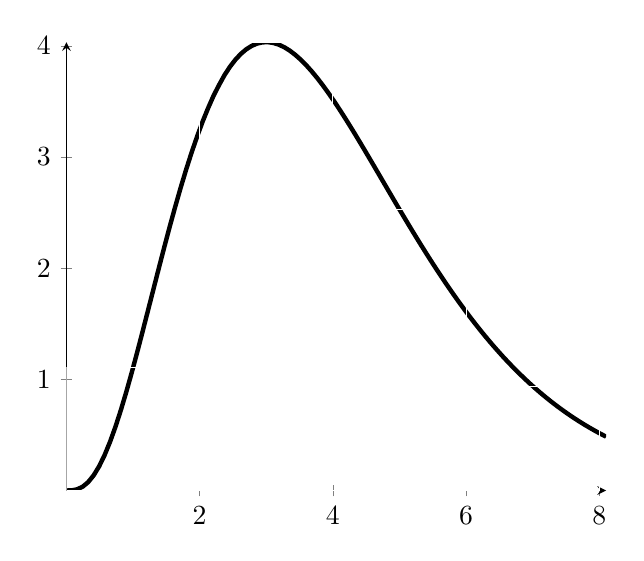
\begin{tikzpicture}[color=black,/pgf/declare function={f=3*e^(-x)*x^3;}]
\begin{axis}[
    domain=0:8.1,
    samples=100,
    axis lines=middle
]
\addplot [ultra thick] {f};
\addplot [
    white,
    integral segments=4,
    integral=0:8
] {f};
\end{axis}
\end{tikzpicture}
\newline \small \textbf{Table II:} Each model was measured by how accurate it was able to correctly classify pull requests. Precision and recall are also used to evaluate the performance of each model.
\end{center}
\end{figure}


\section{Discussion of Results}
\subsection{Research Questions \#1}
Not all attributes are needed in classifying pull requests. However, the naturalness of code and analyzing structural changes has shown strong correlation with accepted pull requests. 

\subsection{Research Question \#2}
We show that fine-grained source code changes in pull request can lead to improved models for predicting pull request acceptance. In Table [insert table number], the basic model received an accuracy rate of 58\% and the advanced model generated a 64\% accuracy rate. With the addition of the behavior presented in Research Question 1, the model was able to predict at a 6\% higher accuracy. Although the basic model was able to recall more accepted pulls compared to the advanced model, the advanced model had a higher precision rate of .06. Based on these results, we can answer the question: Structured behavior of accepted pull request can predict pull request acceptance by creating a model using the Random Forest algorithm.

\subsection{Research Question \# 3}
In our approach, we created various models with the same data but with a unique metric missing. Taking the accuracy of each model, we are able to measure the influence which each metric has on the overall advance model?s accuracy. In our findings, we discovered that [insert how many metrics out of total metrics] presented by the basic model only decreased the overall accuracy rate. As a result of removing these metrics, the accuracy increased from 64\% to 67\%. This could also be due to the model used with the data presented, but we argue that the quality of data has more importance in predicting accuracy than the algorithm of the model. Beyond the metrics found in the basic model, our findings also showed that the entropy metrics and structural changes had the biggest influence over the accuracy rate. The model which excluded entropy metrics had the biggest decrease in accuracy rate of 4\%. We pose that the ?usefulness? of a metric is defined by its positive influence over the overall accuracy We can now answer the third research question: Entropy and structural changes had the most influence over the accuracy of the advanced model.

\section{Conclusion}
Throughout this paper, we analyzed what change occurs in pull requests. The following are the results we have concluded:
R1. High entropy and structural changes are present in accepted pull requests.
R2. The model with the these behavior as performance metrics performed better with a higher accuracy rate.
R3. Entropy and structural changes are also the biggest influence in the model.
This paper also presents the argument that analyzing code at the structural is a better method of collecting data. As this method could be applied to other research questions, measuring the specific elements of code can present better models for prediction or classification of code. Overall, the nature of this project contributes findings to understanding the nature of social computing, specifically OSS. 

\subsection{Threats to Validity}
This project faces one particular threat to its validity. In the nature of bug fixing and the definition of a bug, a pull request acceptance may not indicate whether a pull request fixed a bug. This could alter the collected data and detour from the high-level purpose of the project. However, the advanced model proved to have a high predicting accuracy, this threat may not as be detrimental as we thought. Additional threat to validity includes limiting dataset to just Java projects. It is evident that Java projects are more explicit with its data structure than other programming languages. In terms of practicality, the approach we took may not work for the OSS written in other languages.

\subsection{Future Work}
We hope to expand this work to more programming languages. This would involve understanding Change Distiller?s algorithm and implementing its AST converter to languages like C and Python As the high-level goal is to understand the process of bug fixing in OSS, this work can be expanded to understand the behavior of the fix itself. Furthermore, if common bugs are found, there should be a common solution.

\section*{Acknowledgment}

The authors would like to thank...
more thanks here



\bibliography{mybib}{}
\bibliographystyle{plain}


% that's all folks
\end{document}


